\chapter{Introducción}
El presente Trabajo de Fin de Máster (TFM) se ocupa de resolver una problemática real dentro del campo de la identificación humana. En concreto, se hace uso de métodos de aprendizaje profundo y visión por computador para automatizar una técnica de antropología forense empleada en tareas de estimación del perfil biológico, más específicamente, la estimación de la edad de personas fallecidas a partir de restos óseos. 

Este capítulo introductorio se centra en presentar el problema en detalle, la motivación que nos lleva a enfrentarnos a él y el objetivo principal abordado en este TFM. 


\section{Definición del Problema}
\label{daIntro_ProblemDef}
%Que es la antropología forense
La antropología forense (AF) constituye una disciplina especializada que se dedica al estudio y análisis detallado de restos humanos, específicamente a través de la información obtenida de los huesos, con un propósito médico-legal \cite{byers_introduction_2016,RefWorks:RefID:17-christensen2019forensic}. Este campo combina conocimientos de la antropología física y de otras ramas afines para proporcionar información clave en investigaciones legales.

La antropología física, a su vez, es el campo que estudia la evolución de la especie humana, así como de las condiciones de vida y salud de distintas poblaciones, tanto antiguas como contemporáneas, mediante estudios osteológicos (del hueso) y somatológicos (del cuerpo). Este conocimiento no solo permite un análisis detallado de los restos óseos, sino que también incluye una comprensión integral de los aspectos sociales, culturales y de comportamiento humano \cite{antrofisica}. Los expertos en AF, a través de este enfoque multidisciplinario, examinan minuciosamente los restos óseos para extraer la mayor cantidad posible de información relevante, la cual se utiliza para lograr los siguientes objetivos:

\begin{enumerate}
    \item Establecer la ascendencia y las características morfológicas del fallecido.
    \item Identificar las circunstancias y el modo en que ocurrió la muerte de la persona.
    \item Determinar el tiempo transcurrido desde el fallecimiento.
    \item Colaborar en la recuperación de restos, tanto superficiales como enterrados, que sean de interés para la investigación forense.
    \item Proporcionar información útil para la identificación de personas fallecidas, basándose en las características morfológicas presentes en los huesos humanos.
    \item Analizar el esqueleto de personas vivas con fines médico-legales, como en el caso de la identificación de migrantes o menores desaparecidos.
\end{enumerate}

La estimación del perfil biológico (PB) constituye una de las áreas fundamentales de la AF, ya que se enfoca en la identificación de características clave de los restos óseos. Este proceso incluye la determinación de la edad, el sexo, la estatura y el origen poblacional o ascendencia, además de cualquier otra particularidad que ayude a individualizar los restos, ya sea total o parcialmente esqueletizados. La finalidad de esta evaluación es facilitar la búsqueda de la identidad de una persona desaparecida y, de ser posible, lograr una identificación positiva y certera. Un esquema ilustrativo del proceso de identificación forense puede apreciarse en la Figura \ref{fig:intro_1}.

\begin{figure}[h]
    \centering
    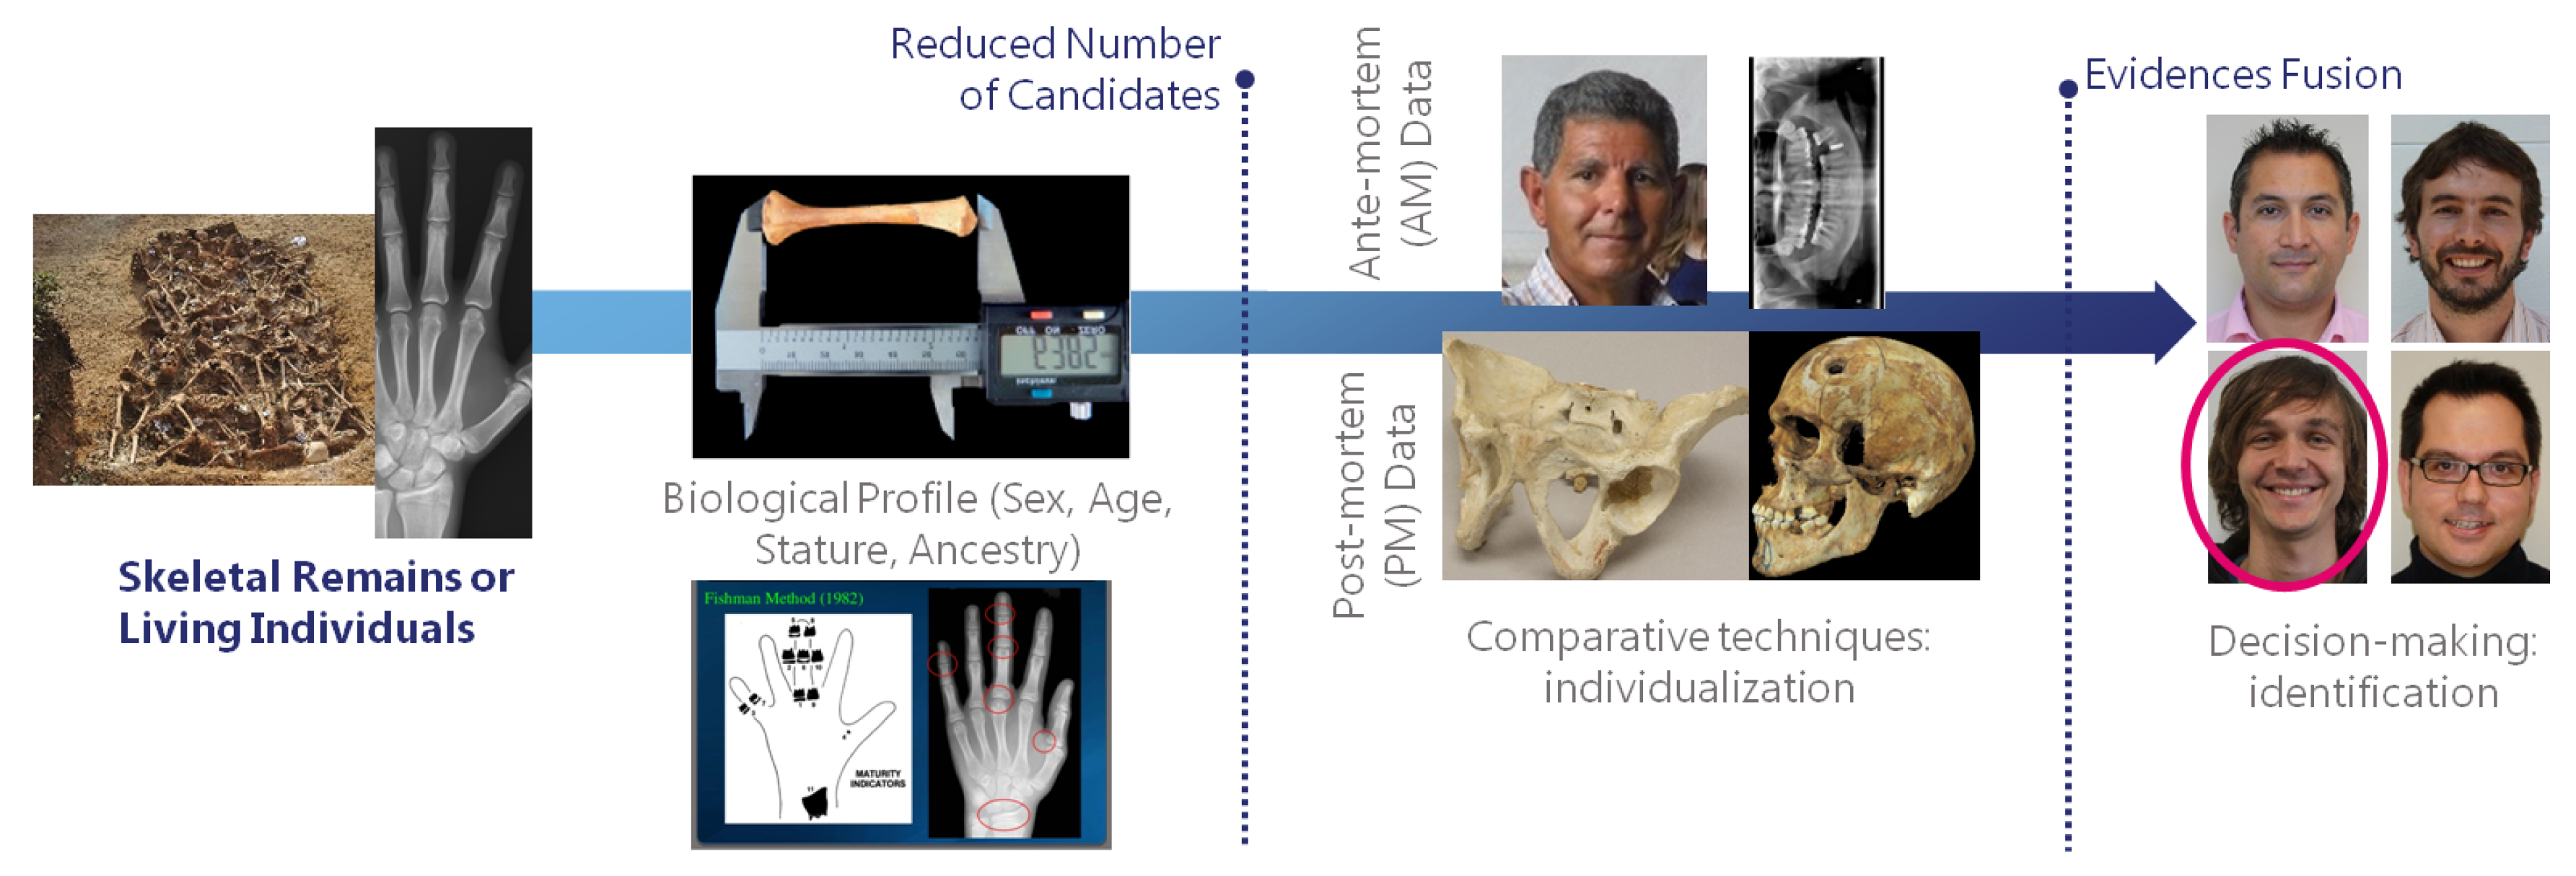
\includegraphics[width=1\linewidth]{figures/1_introduction/intro_1.png}
    \caption[Proceso de identificación forense a partir de restos óseos]{Proceso de identificación forense a partir de restos óseos \cite{RefWorks:RefID:21-mesejo2020survey}.}
    \label{fig:intro_1}
\end{figure}

Uno de los aspectos fundamentales en la elaboración del PB es la estimación de la edad de los restos. Para lograrlo, se examinan estructuras como las suturas craneales \cite{skullAF}, las costillas \cite{icscan1984age}, la cara auricular del ilion \cite{buckberry_age_2002} y la sínfisis del pubis, estos dos últimos localizados en la pelvis. En cada caso, se observa el grado de desgaste que presentan estos huesos en el momento del fallecimiento, lo cual permite aproximarse a la edad del individuo \cite{RefWorks:RefID:12-black2011forensic}.

La sínfisis del pubis es el hueso más utilizado para estimar la edad de un individuo, siendo la opción preferida por el 95\% de los antropólogos forenses \cite{garvin_current_2012}. El método predominante se fundamenta en el trabajo pionero de Thomas Wingate Todd \cite{RefWorks:RefID:19-todd1921age}, quien en 1921 documentó las transformaciones progresivas de la sínfisis del pubis con el envejecimiento, permitiendo estimar un rango aproximado de edad al momento del fallecimiento. Todd propuso un sistema de etapas de envejecimiento que ha sido revisado y perfeccionado en múltiples ocasiones; la revisión más reconocida corresponde al método de Suchey-Brooks \cite{RefWorks:RefID:20-brooks1990skeletal}, publicado en 1990. Este enfoque se basa en el análisis de nueve características específicas de la sínfisis del pubis y, en función del estado de cada una, asigna atributos categóricos que reflejan el grado de erosión ósea en distintas áreas, permitiendo así calcular un rango estimado de edad para el difunto. Dichas características se detallan en la Tabla \ref{table:themBones}, y en la Tabla \ref{themBomes:visualExample} se presenta un ejemplo visual de cada una de ellas.

\begin{table}[h]
\resizebox{\textwidth}{!}{%
\begin{tabular}{c|ll}
\hline
\multicolumn{1}{|c|}{\cellcolor[HTML]{FFC702}\textbf{Característica}} & \multicolumn{2}{c|}{\cellcolor[HTML]{FFC702}\textbf{Atributo}} \\ \hline
\multicolumn{1}{|c|}{\textbf{\textit{Crestas y Surcos}}} & \multicolumn{1}{l|}{Porosidad Regular} & \multicolumn{1}{l|}{Muy Definidas} \\ \hline
 & \multicolumn{1}{l|}{Poco Profundas} & \multicolumn{1}{l|}{Restos de Surcos} \\ \cline{2-3} 
 & \multicolumn{1}{l|}{No hay Surcos} &  \\ \hline
\multicolumn{1}{|c|}{\textbf{\textit{Porosidad Irregular}}} & \multicolumn{1}{l|}{No} & \multicolumn{1}{l|}{Mediana} \\ \hline
 & \multicolumn{1}{l|}{Sí} &  \\ \hline
\multicolumn{1}{|c|}{\textbf{\textit{Borde Superior}}} & \multicolumn{1}{l|}{No Definido} & \multicolumn{1}{l|}{Definido} \\ \hline
\multicolumn{1}{|c|}{\textbf{\textit{Nódulo Óseo}}} & \multicolumn{1}{l|}{Ausente} & \multicolumn{1}{l|}{Presente} \\ \hline
\multicolumn{1}{|c|}{\textbf{\textit{Borde Inferior}}} & \multicolumn{1}{l|}{No Definido} & \multicolumn{1}{l|}{Definido} \\ \hline
\multicolumn{1}{|c|}{\textbf{\textit{Borde Dorsal}}} & \multicolumn{1}{l|}{No Definido} & \multicolumn{1}{l|}{Definido} \\ \hline
\multicolumn{1}{|c|}{\textbf{\textit{Plataforma Dorsal}}} & \multicolumn{1}{l|}{Ausente} & \multicolumn{1}{l|}{Presente} \\ \hline
\multicolumn{1}{|c|}{\textbf{\textit{Bisel Ventral}}} & \multicolumn{1}{l|}{Ausente} & \multicolumn{1}{l|}{En Formación} \\ \hline
 & \multicolumn{1}{l|}{Presente} &  \\ \hline
\multicolumn{1}{|c|}{\textbf{\textit{Borde Ventral}}} & \multicolumn{1}{l|}{Ausente} & \multicolumn{1}{l|}{En Formación} \\ \hline
 & \multicolumn{1}{l|}{Formado, Sin Excrecencias} & \multicolumn{1}{l|}{Formado, Pocas Excrecencias} \\ \cline{2-3} 
 & \multicolumn{1}{l|}{Formado, Muchas Excrecencias} &  \\ \cline{2-2}
\end{tabular}%
}
\caption[Método de Todd: Características para determinación de edad]{Características utilizadas para la determinación de la edad según el método de Todd \cite{RefWorks:RefID:19-todd1921age} y sus derivados.}
\label{table:themBones}
\end{table}

\begin{table}[h]
\centering
\resizebox{\textwidth}{!}{%
\begin{tabular}{|
>{\columncolor[HTML]{FFC702}}c|c|c|c|c|c|c|c|}
\hline
\textbf{Característica} & \textit{\textbf{\begin{tabular}[c]{@{}c@{}}Crestas y \\ Surcos\end{tabular}}} & \textit{\textbf{\begin{tabular}[c]{@{}c@{}}Porosidad \\ Irregular\end{tabular}}} & \textit{\textbf{\begin{tabular}[c]{@{}c@{}}Borde \\ Superior\end{tabular}}} & \textit{\textbf{\begin{tabular}[c]{@{}c@{}}Nódulo \\ Óseo\end{tabular}}} & \textit{\textbf{\begin{tabular}[c]{@{}c@{}}Borde \\ Inferior\end{tabular}}} & \textit{\textbf{\begin{tabular}[c]{@{}c@{}}Borde \\ Dorsal\end{tabular}}} & \textit{\textbf{\begin{tabular}[c]{@{}c@{}}Plataforma \\ Dorsal\end{tabular}}} \\ \hline
\textbf{Atributo} & Muy Definidos & Sí & Definido & Presente & Definido & Definido & Presente \\ \hline
\textbf{Ejemplo} & 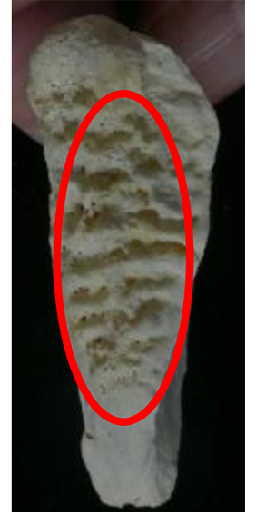
\includegraphics[align=c, width=0.2\linewidth]{figures/1_introduction/todd1.png} & 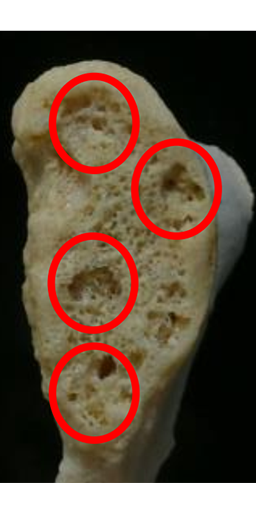
\includegraphics[align=c, width=0.2\linewidth]{figures/1_introduction/todd2.png} & 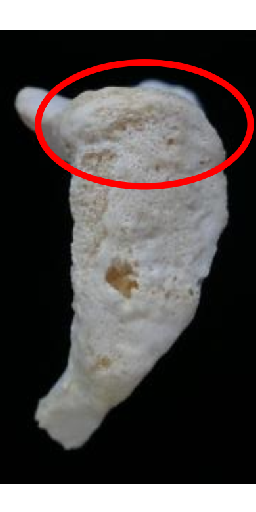
\includegraphics[align=c, width=0.2\linewidth]{figures/1_introduction/todd3.png} & 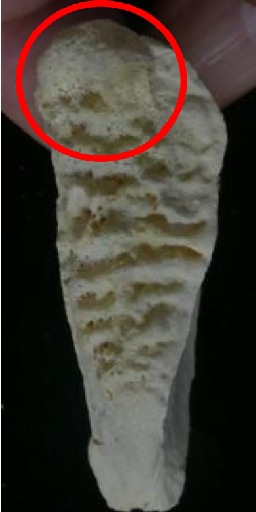
\includegraphics[align=c, width=0.2\linewidth]{figures/1_introduction/todd4.png} & 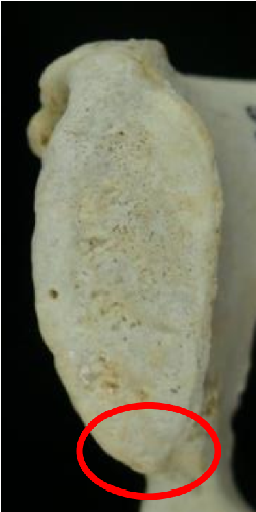
\includegraphics[align=c, width=0.2\linewidth]{figures/1_introduction/todd5.png} & 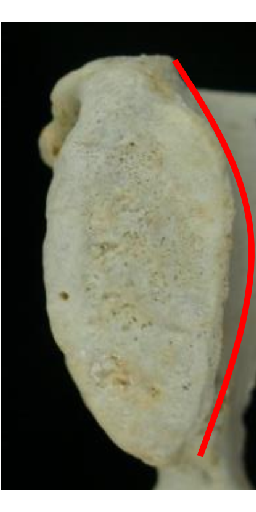
\includegraphics[align=c, width=0.2\linewidth]{figures/1_introduction/todd6.png} & 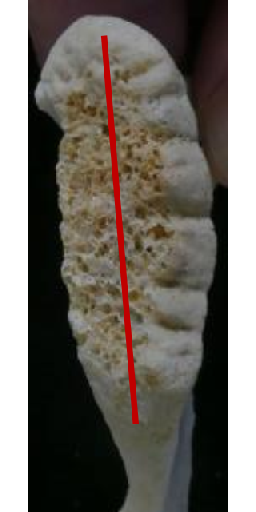
\includegraphics[align=c, width=0.2\linewidth]{figures/1_introduction/todd7.png} \\ \hline
\end{tabular}%
}
\caption[Método de Todd: Ejemplo de características]{Ejemplo de las características del método de Todd y sus derivados.}
\label{themBomes:visualExample}
\end{table}

Es importante destacar que la metodología empleada en este método, al igual que en muchas otras de la AF, depende en gran medida del criterio subjetivo del experto. Esto genera errores intraevaluador e interevaluador, ya que el uso de criterios subjetivos y descriptivos introduce limitaciones debido a las diversas interpretaciones entre evaluadores \cite{RefWorks:RefID:12-black2011forensic}. Tal situación disminuye la confiabilidad y validez de los resultados obtenidos, lo que finalmente reduce la credibilidad de los estudios forenses cuando se presentan como evidencia en un juicio. Esta problemática justifica la búsqueda de herramientas y metodologías que, al menos parcialmente, mitiguen dichas limitaciones. En este contexto, disciplinas como la inteligencia artificial (IA) y, en particular, el aprendizaje automático (\textit{Machine Learning}, ML) \cite{abu-mostafa_learning_2012, mitchell_introduction_1997}, el aprendizaje profundo (\textit{Deep Learning}, DL) \cite{Goodfellow-et-al-2016, chollet_deep_2021} y la visión por computador (\textit{Computer Vision}, CV) pueden asistir, automatizar y acelerar las tareas forenses, reduciendo significativamente los sesgos y errores.

Considerando todo lo anterior, el presente TFM se centra en la clasificación automática de las características morfológicas de la sínfisis del pubis para estimar la edad a partir de modelos 3D mediante técnicas de IA.

\section{Motivación}
En las últimas décadas, la IA ha facilitado la automatización de tareas repetitivas y tediosas para los humanos, así como la superación de la capacidad humana en actividades complejas, particularmente en los campos de ML y CV. En estos ámbitos, se han logrado avances significativos en tareas como la detección, generación y restauración de imágenes \cite{krizhevsky_imagenet_2017}. Estas técnicas han sido ampliamente adoptadas en diversas disciplinas, incluida la medicina, donde han proporcionado herramientas de gran utilidad para los profesionales del área.

No obstante, resulta sorprendente que, en la actualidad, la AF siga presentando un nivel relativamente bajo de sofisticación tecnológica \cite{RefWorks:RefID:21-mesejo2020survey}. En este contexto, una de las principales motivaciones de este trabajo es impulsar la modernización y automatización de la AF desde una perspectiva tecnológica, centrándose particularmente en la aplicación de técnicas avanzadas para la estimación de edad.

Además, como se mencionó previamente, la subjetividad inherente a la antropología forense representa un desafío desde el punto de vista legal. En muchos casos, los análisis carecen de una base científica sólida según el criterio de Daubert \cite{noauthor_daubert_nodate}, el cual establece los requisitos para la admisibilidad del testimonio experto en un juicio. Según este criterio, un método es válido si: (1) los resultados son reproducibles y han sido verificados por terceros, (2) posee tasas de error conocidas y (3) es aceptado por la comunidad científica forense.

En este sentido, la aplicación de IA en antropología forense puede contribuir significativamente a la reducción de la subjetividad en las identificaciones, minimizando errores humanos, automatizando múltiples tareas, estructurando el conocimiento experto y facilitando la obtención de nuevos hallazgos. Esto, a su vez, fortalecería la base científica de los métodos utilizados en la disciplina, permitiendo que sean reproducibles y que se conozcan con precisión sus tasas de error, lo que favorecería su cumplimiento con el criterio de Daubert y su aceptación en el ámbito legal.

Si se analiza el contexto global de la identificación humana, se evidencia que la estimación del PB mediante técnicas de AF adquiere especial relevancia, puesto que otras herramientas de mayor precisión y sofisticación, como el análisis de ADN o la toma de huellas dactilares, presentan limitaciones significativas. Por ejemplo, el análisis de ADN requiere una inversión elevada en recursos y tiempo, y al igual que la obtención de huellas dactilares, depende de la disponibilidad de datos tanto ante-mortem como post-mortem. Además, ambas técnicas se ven afectadas por el estado de los tejidos blandos, que son los más susceptibles a la descomposición natural o a daños provocados por quemaduras, exposición a agua, productos químicos, entre otros factores. En cambio, el tejido óseo, en general, demuestra una mayor resistencia y es frecuentemente lo único recuperable tras la completa descomposición de los tejidos blandos. Por ello, las técnicas basadas en AF son especialmente útiles en los siguientes escenarios:
\begin{itemize}
    \item Identificación masiva de víctimas de desastres naturales, accidentes o ataques terroristas.
    \item Identificación de víctimas de conflictos armados o actos de lesa humanidad, donde los restos pueden estar desmembrados, desfigurados y/o quemados.
    \item Procesamiento de fosas comunes en las que los restos óseos se han mezclado.
    \item Identificación de personas desaparecidas en contextos no relacionados con desastres o guerras, en los que las condiciones del cadáver han impedido la aplicación de otras técnicas \cite{byers_introduction_2016}.
\end{itemize}

Para dimensionar el desafío al que se enfrentan los antropólogos forenses, es relevante considerar que, únicamente en el año 2019, 20 000 personas perdieron la vida por causas vinculadas al terrorismo, con un promedio anual de 24 000 muertes en la última década atribuibles a este fenómeno \cite{owid_terrorism}. Asimismo, los desastres naturales ocasionan aproximadamente entre 40 000 y 50 000 muertes anuales \cite{owid_natural_disasters}. En el caso de Ucrania, al momento de la redacción de este documento, se contabilizan más de 60 000 personas desaparecidas, entre las que se incluyen víctimas no identificadas de la guerra, residentes de las zonas ocupadas al este del país, y posibles víctimas derivadas del impacto del intenso frío en áreas sin suministro eléctrico \cite{blanco_ucrania_2024}. En España, aún se deben recuperar alrededor de 20 000 víctimas de la Guerra Civil, muchas de las cuales se hallan en fosas y cunetas, de modo que apenas un tercio de ellas podría ser identificada mediante análisis de ADN \cite{junquera_huellas_2022}.

Estos datos subrayan la imperiosa necesidad de incorporar técnicas informáticas automatizadas en el ámbito de la AF, ya que permitirían una considerable optimización en términos de tiempo y recursos, facilitando la detección de las características determinantes para la estimación de la edad en situaciones en las que el número de individuos a identificar es elevado y otras técnicas no son aplicables.

\section{Objetivos}
Tras haber descrito el problema y su motivación, el objetivo principal de este TFM consiste en desarrollar y validar un modelo de aprendizaje profundo que utilice modelos 3D de la sínfisis púbica. Este modelo tiene como finalidad extraer características morfológicas relevantes de dicho hueso, contribuyendo así a la automatización de la estimación de la edad en el ámbito de la antropología forense.

Este objetivo principal se desglosa en los siguientes objetivos parciales:
\begin{enumerate}
    \item Estudio pormenorizado de la literatura relativa a la estimación de edad a partir de restos óseos, y al procesado de modelos 3D por medio de redes neuronales profundas.
    \item Análisis y discusión de los modelos existentes, y selección razonada de los candidatos más prometedores para el problema actual.
    \item Creación de un prototipo y validación experimental con modelos 3D de la sínfisis del pubis.
    \item Extracción de una o varias de las más relevantes características para poder llevar a cabo la estimación de la edad. 
\end{enumerate}
